\documentclass[]{article}
\usepackage{lmodern}
\usepackage{amssymb,amsmath}
\usepackage{ifxetex,ifluatex}
\usepackage{fixltx2e} % provides \textsubscript
\ifnum 0\ifxetex 1\fi\ifluatex 1\fi=0 % if pdftex
  \usepackage[T1]{fontenc}
  \usepackage[utf8]{inputenc}
\else % if luatex or xelatex
  \ifxetex
    \usepackage{mathspec}
  \else
    \usepackage{fontspec}
  \fi
  \defaultfontfeatures{Ligatures=TeX,Scale=MatchLowercase}
\fi
% use upquote if available, for straight quotes in verbatim environments
\IfFileExists{upquote.sty}{\usepackage{upquote}}{}
% use microtype if available
\IfFileExists{microtype.sty}{%
\usepackage{microtype}
\UseMicrotypeSet[protrusion]{basicmath} % disable protrusion for tt fonts
}{}
\usepackage[margin=1in]{geometry}
\usepackage{hyperref}
\hypersetup{unicode=true,
            pdftitle={Song Key Mode \& Popularity},
            pdfauthor={Socorro Dominguez and Paul Vial},
            pdfborder={0 0 0},
            breaklinks=true}
\urlstyle{same}  % don't use monospace font for urls
\usepackage{longtable,booktabs}
\usepackage{graphicx,grffile}
\makeatletter
\def\maxwidth{\ifdim\Gin@nat@width>\linewidth\linewidth\else\Gin@nat@width\fi}
\def\maxheight{\ifdim\Gin@nat@height>\textheight\textheight\else\Gin@nat@height\fi}
\makeatother
% Scale images if necessary, so that they will not overflow the page
% margins by default, and it is still possible to overwrite the defaults
% using explicit options in \includegraphics[width, height, ...]{}
\setkeys{Gin}{width=\maxwidth,height=\maxheight,keepaspectratio}
\IfFileExists{parskip.sty}{%
\usepackage{parskip}
}{% else
\setlength{\parindent}{0pt}
\setlength{\parskip}{6pt plus 2pt minus 1pt}
}
\setlength{\emergencystretch}{3em}  % prevent overfull lines
\providecommand{\tightlist}{%
  \setlength{\itemsep}{0pt}\setlength{\parskip}{0pt}}
\setcounter{secnumdepth}{0}
% Redefines (sub)paragraphs to behave more like sections
\ifx\paragraph\undefined\else
\let\oldparagraph\paragraph
\renewcommand{\paragraph}[1]{\oldparagraph{#1}\mbox{}}
\fi
\ifx\subparagraph\undefined\else
\let\oldsubparagraph\subparagraph
\renewcommand{\subparagraph}[1]{\oldsubparagraph{#1}\mbox{}}
\fi

%%% Use protect on footnotes to avoid problems with footnotes in titles
\let\rmarkdownfootnote\footnote%
\def\footnote{\protect\rmarkdownfootnote}

%%% Change title format to be more compact
\usepackage{titling}

% Create subtitle command for use in maketitle
\newcommand{\subtitle}[1]{
  \posttitle{
    \begin{center}\large#1\end{center}
    }
}

\setlength{\droptitle}{-2em}

  \title{Song Key Mode \& Popularity}
    \pretitle{\vspace{\droptitle}\centering\huge}
  \posttitle{\par}
    \author{Socorro Dominguez and Paul Vial}
    \preauthor{\centering\large\emph}
  \postauthor{\par}
      \predate{\centering\large\emph}
  \postdate{\par}
    \date{2018-11-16}

\usepackage{float}

\begin{document}
\maketitle

Is the popularity of songs in a major key different than songs in a
minor key? (Are they more likely to be in the Top 100?) This is the
question we will try to answer by looking at and analyzing Spotify's Top
100 streamed songs!

First of all, in music, ``keys'' are sets of notes which sound
harmonious together. One of the most distinguishing features of a
musical key is its ``mode'' which we can categorize as ``major'' or
``minor.'' These two modes affect the mood of music similarly to how
certain beats may make songs more ``likeable.'' Music written in a major
key-mode usually sounds happy, while music written in a minor key-mode
usually sounds sad or serious. We are interested in whether these modes
(major vs.~minor) of songs' keys affect their popularity.

Spotify is a music streaming platform. They have become an important
platform as they currently have 191 million users. 87 million of these
users, pay in order to be premium users. Their Top 100 is defined by the
songs that are streamed the most throught a year.

Through this evaluation, we go through Spotify's Top 100 2017 data set
to analyze whether people are actively listening to more songs that are
in major key-modes or minor key-modes.

Once we load the data, we make a small summary to see actually how many
songs in Spotify have a minor or a major mode.

Table 1: Summary of how many songs have a major or minor mode:

\begin{longtable}[]{@{}llll@{}}
\toprule
Mode & Avg Rank & Count & Diff. Est.\tabularnewline
\midrule
\endhead
Minor & 48.78 & 42 & 2.9556\tabularnewline
Major & 51.74 & 58 & 2.9556\tabularnewline
\bottomrule
\end{longtable}

We can read from the following graph, that at least for the 2017's Top
100, songs in a major key-mode (or happier sound) were more popular than
songs in a minor key-mode (or sad/serious sound). However, this might
just be by chance.

\begin{figure}[H]
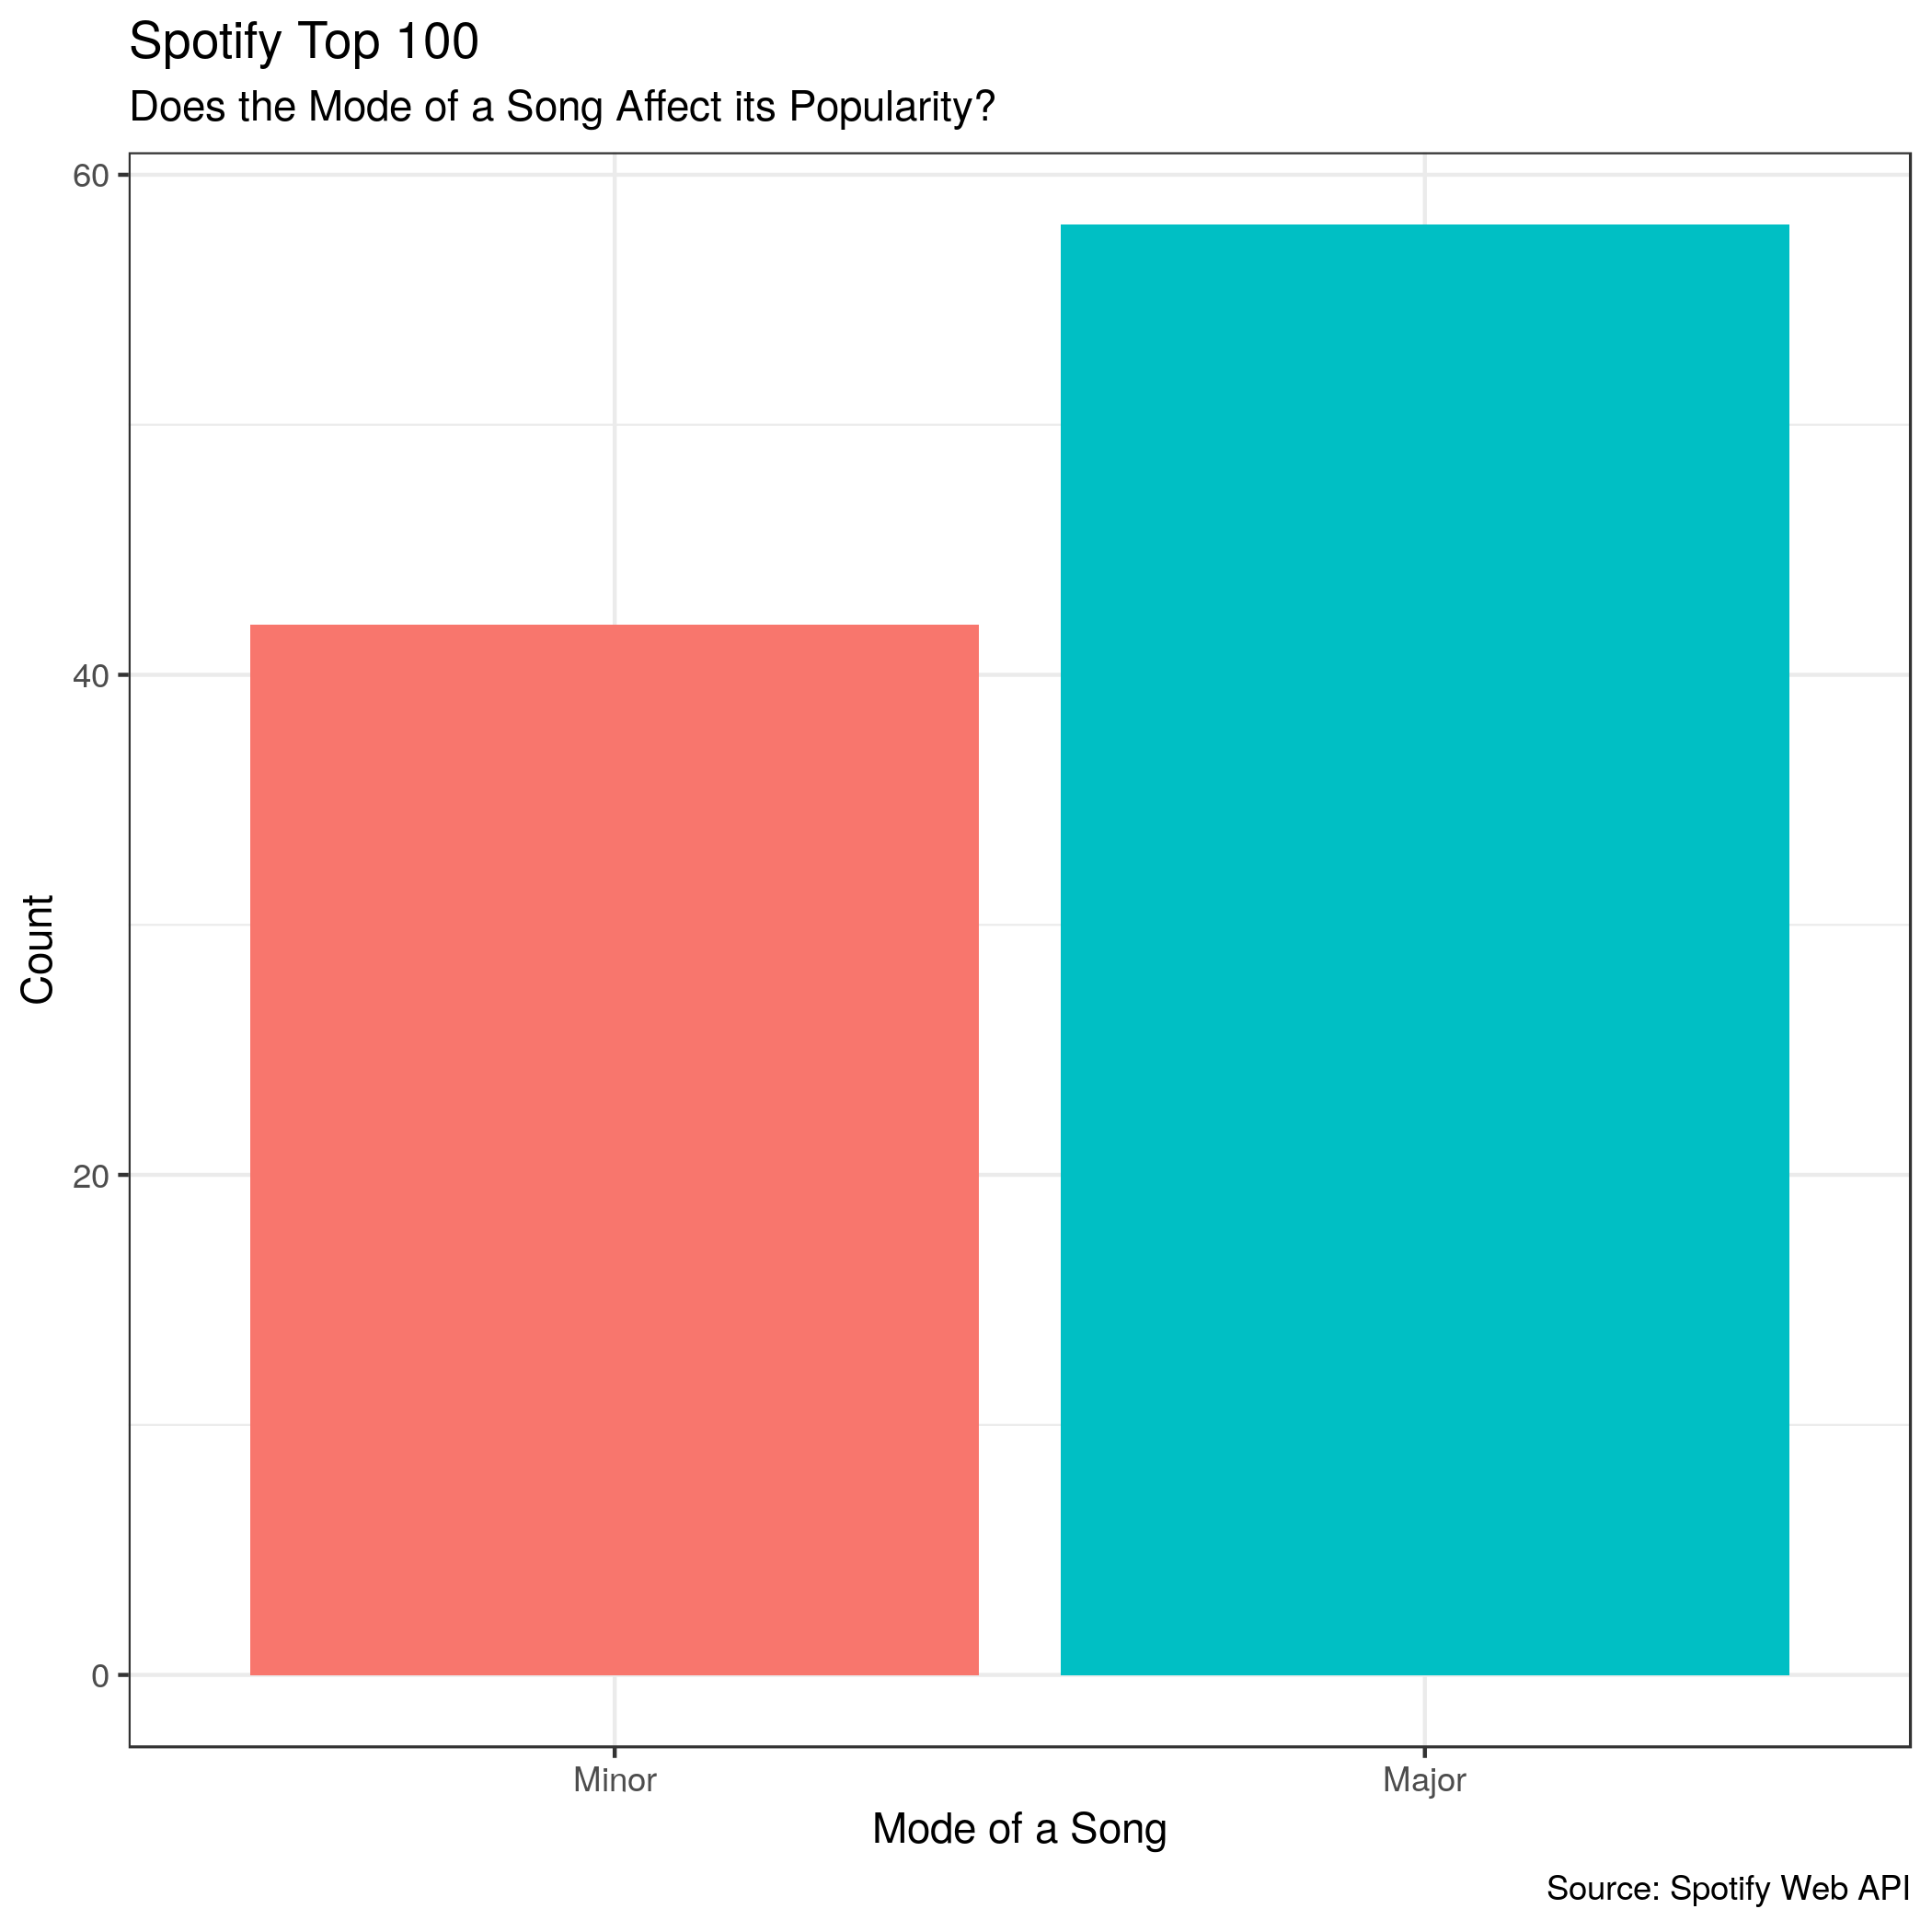
\includegraphics[width=0.8\linewidth]{../results/figure/Fig01_Mode_Viz} \caption{Number of top 100 songs written in each key-mode}\label{fig:unnamed-chunk-1}
\end{figure}

The next plot shows distribution of key-modes throughout the song
rankings that we used. From this visualization we can see that there
does not appear to be any significant clustering of one of the key modes
near a particular range of the song rankings which might affect our
analysis.

\begin{figure}[H]
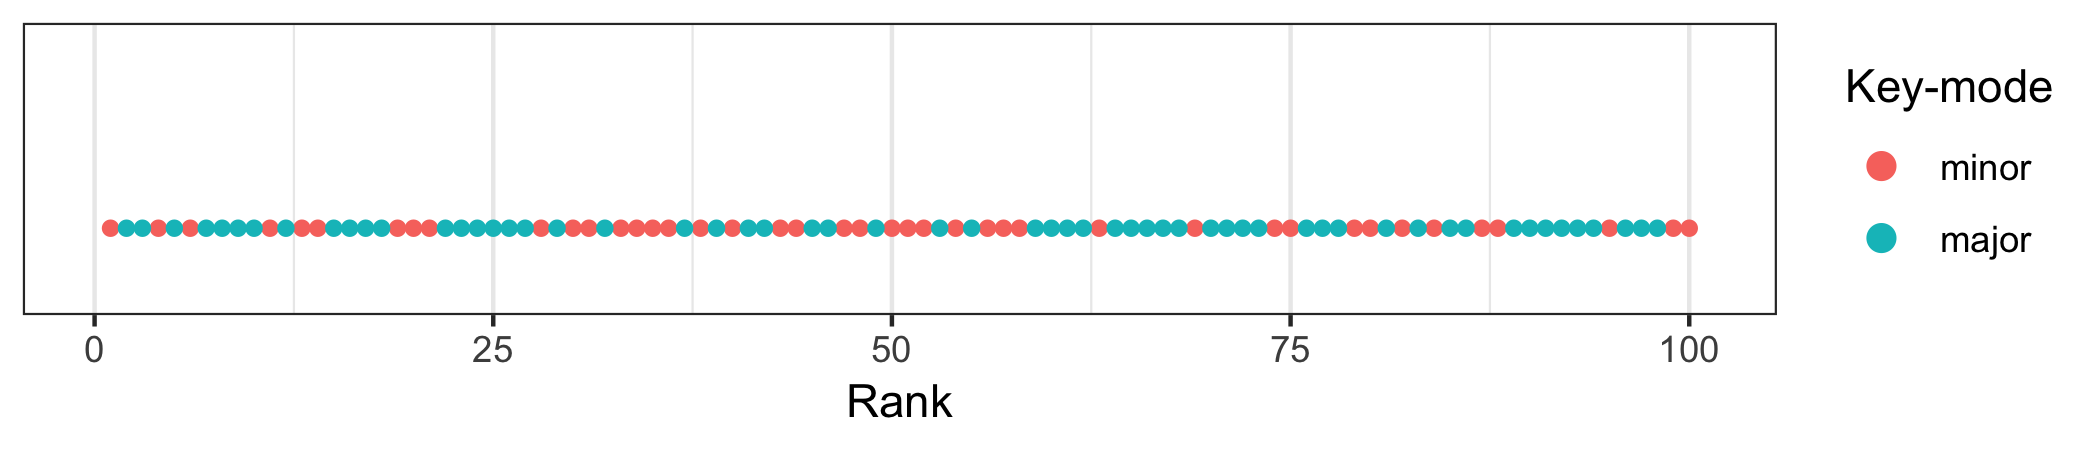
\includegraphics[width=1\linewidth]{../results/figure/Fig05_Mode_Over_Rank_Plot} \caption{Distribution of key-mode over song ranks}\label{fig:unnamed-chunk-2}
\end{figure}

Out of curiousity, let's also evaluate how other features (danceability,
key, loudness, etc) in the song vary with by songs' key-modes:

\begin{figure}[H]
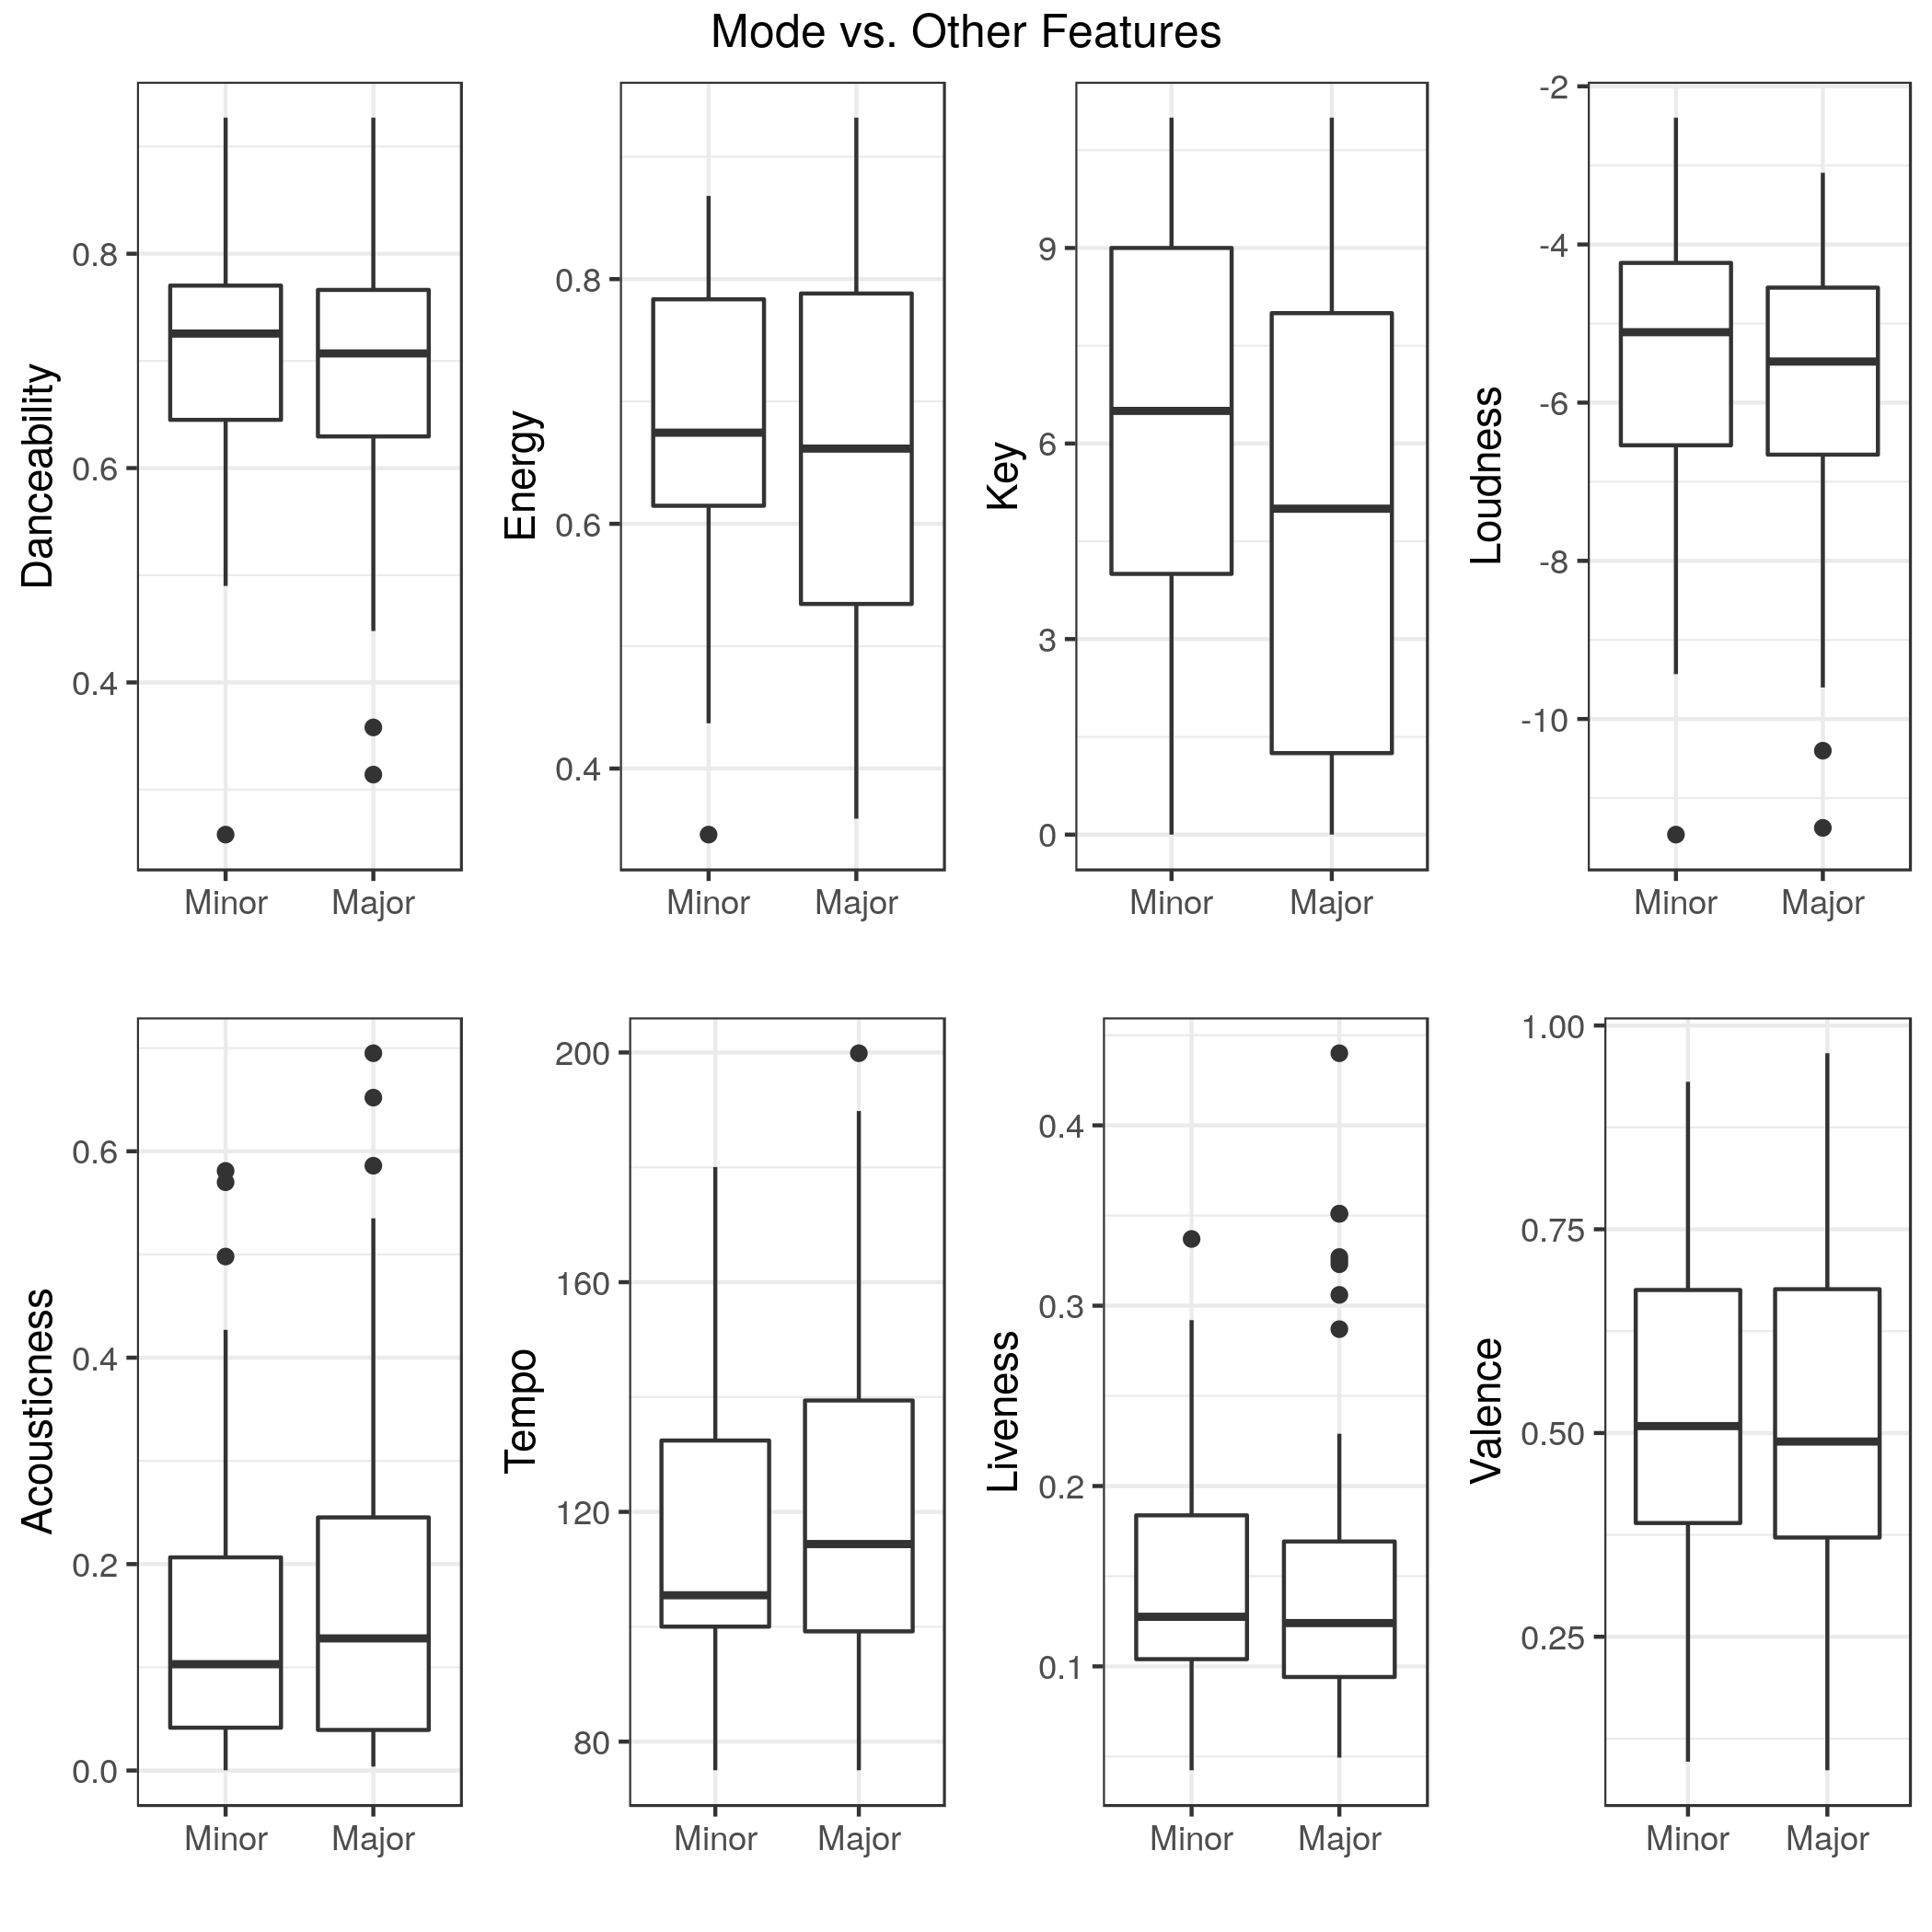
\includegraphics[width=0.8\linewidth]{../results/figure/Fig02_Explore_Mode_and_Features} \caption{ }\label{fig:unnamed-chunk-3}
\end{figure}

We understand, that by just working with this key-mode (rather than the
combination of features) is a limitation of our work. And if given more
time, we would love to explore all the features to see what makes a song
really popular.

Now, using `Estimation through simulation,' we are going to test if the
key-mode actually plays a role in the songs' rankings.

Our hypotheses are as follows:

\textbf{$H_{0}$}: Songs in a major key-mode have an equal average
Spotify ranking to songs in a minor key-mode.

\textbf{$H_{A}$}: Songs in a major key-mode have different average
Spotify ranking than songs in a minor key-mode.

Our test statistic is the difference between songs in a major key-mode
and songs in a minor key-mode.

\begin{figure}[H]
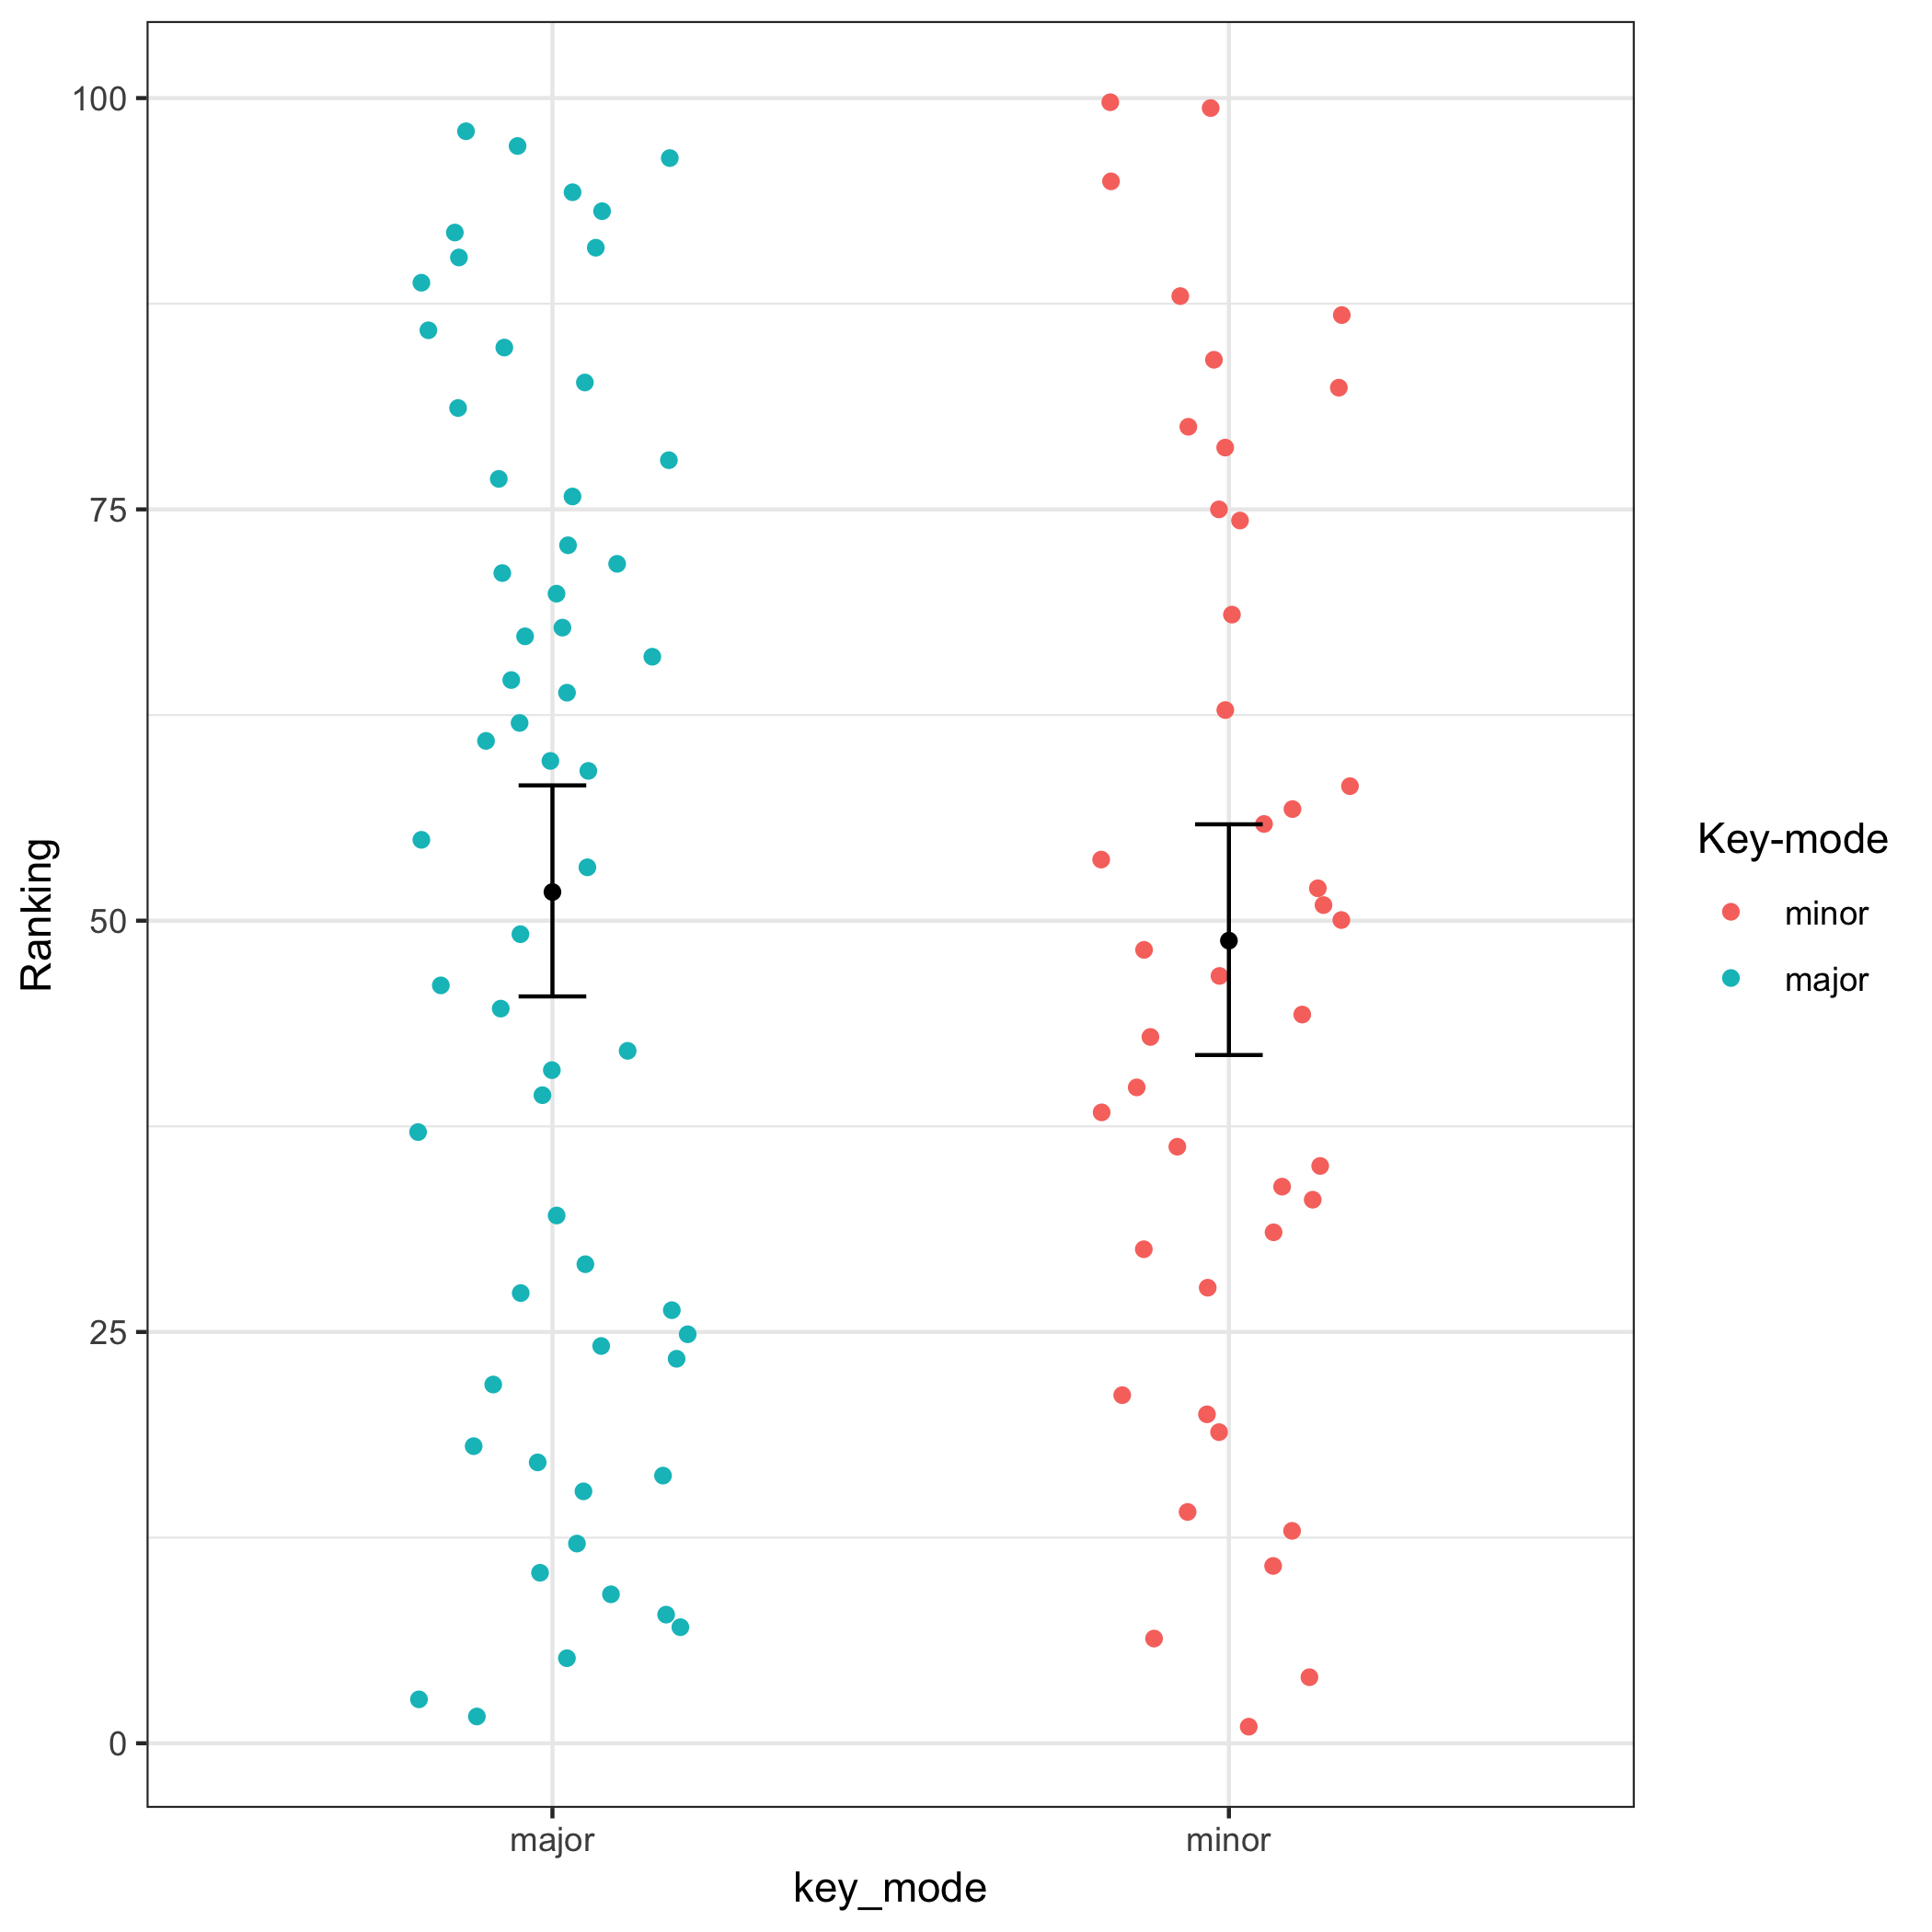
\includegraphics[width=0.8\linewidth]{../results/figure/Fig04_Sample_Compare_Plot} \caption{Error bars represent 95\% confidence intervals generated by bootstrapping}\label{fig:unnamed-chunk-4}
\end{figure}

In the Figure 4 above, we can see that there is significant overlap
between the confidence intervals for the two groups.

Figure 5 below, illustrates where our p-value falls relative to the
confidence interval for our test statistic:

\begin{figure}[H]
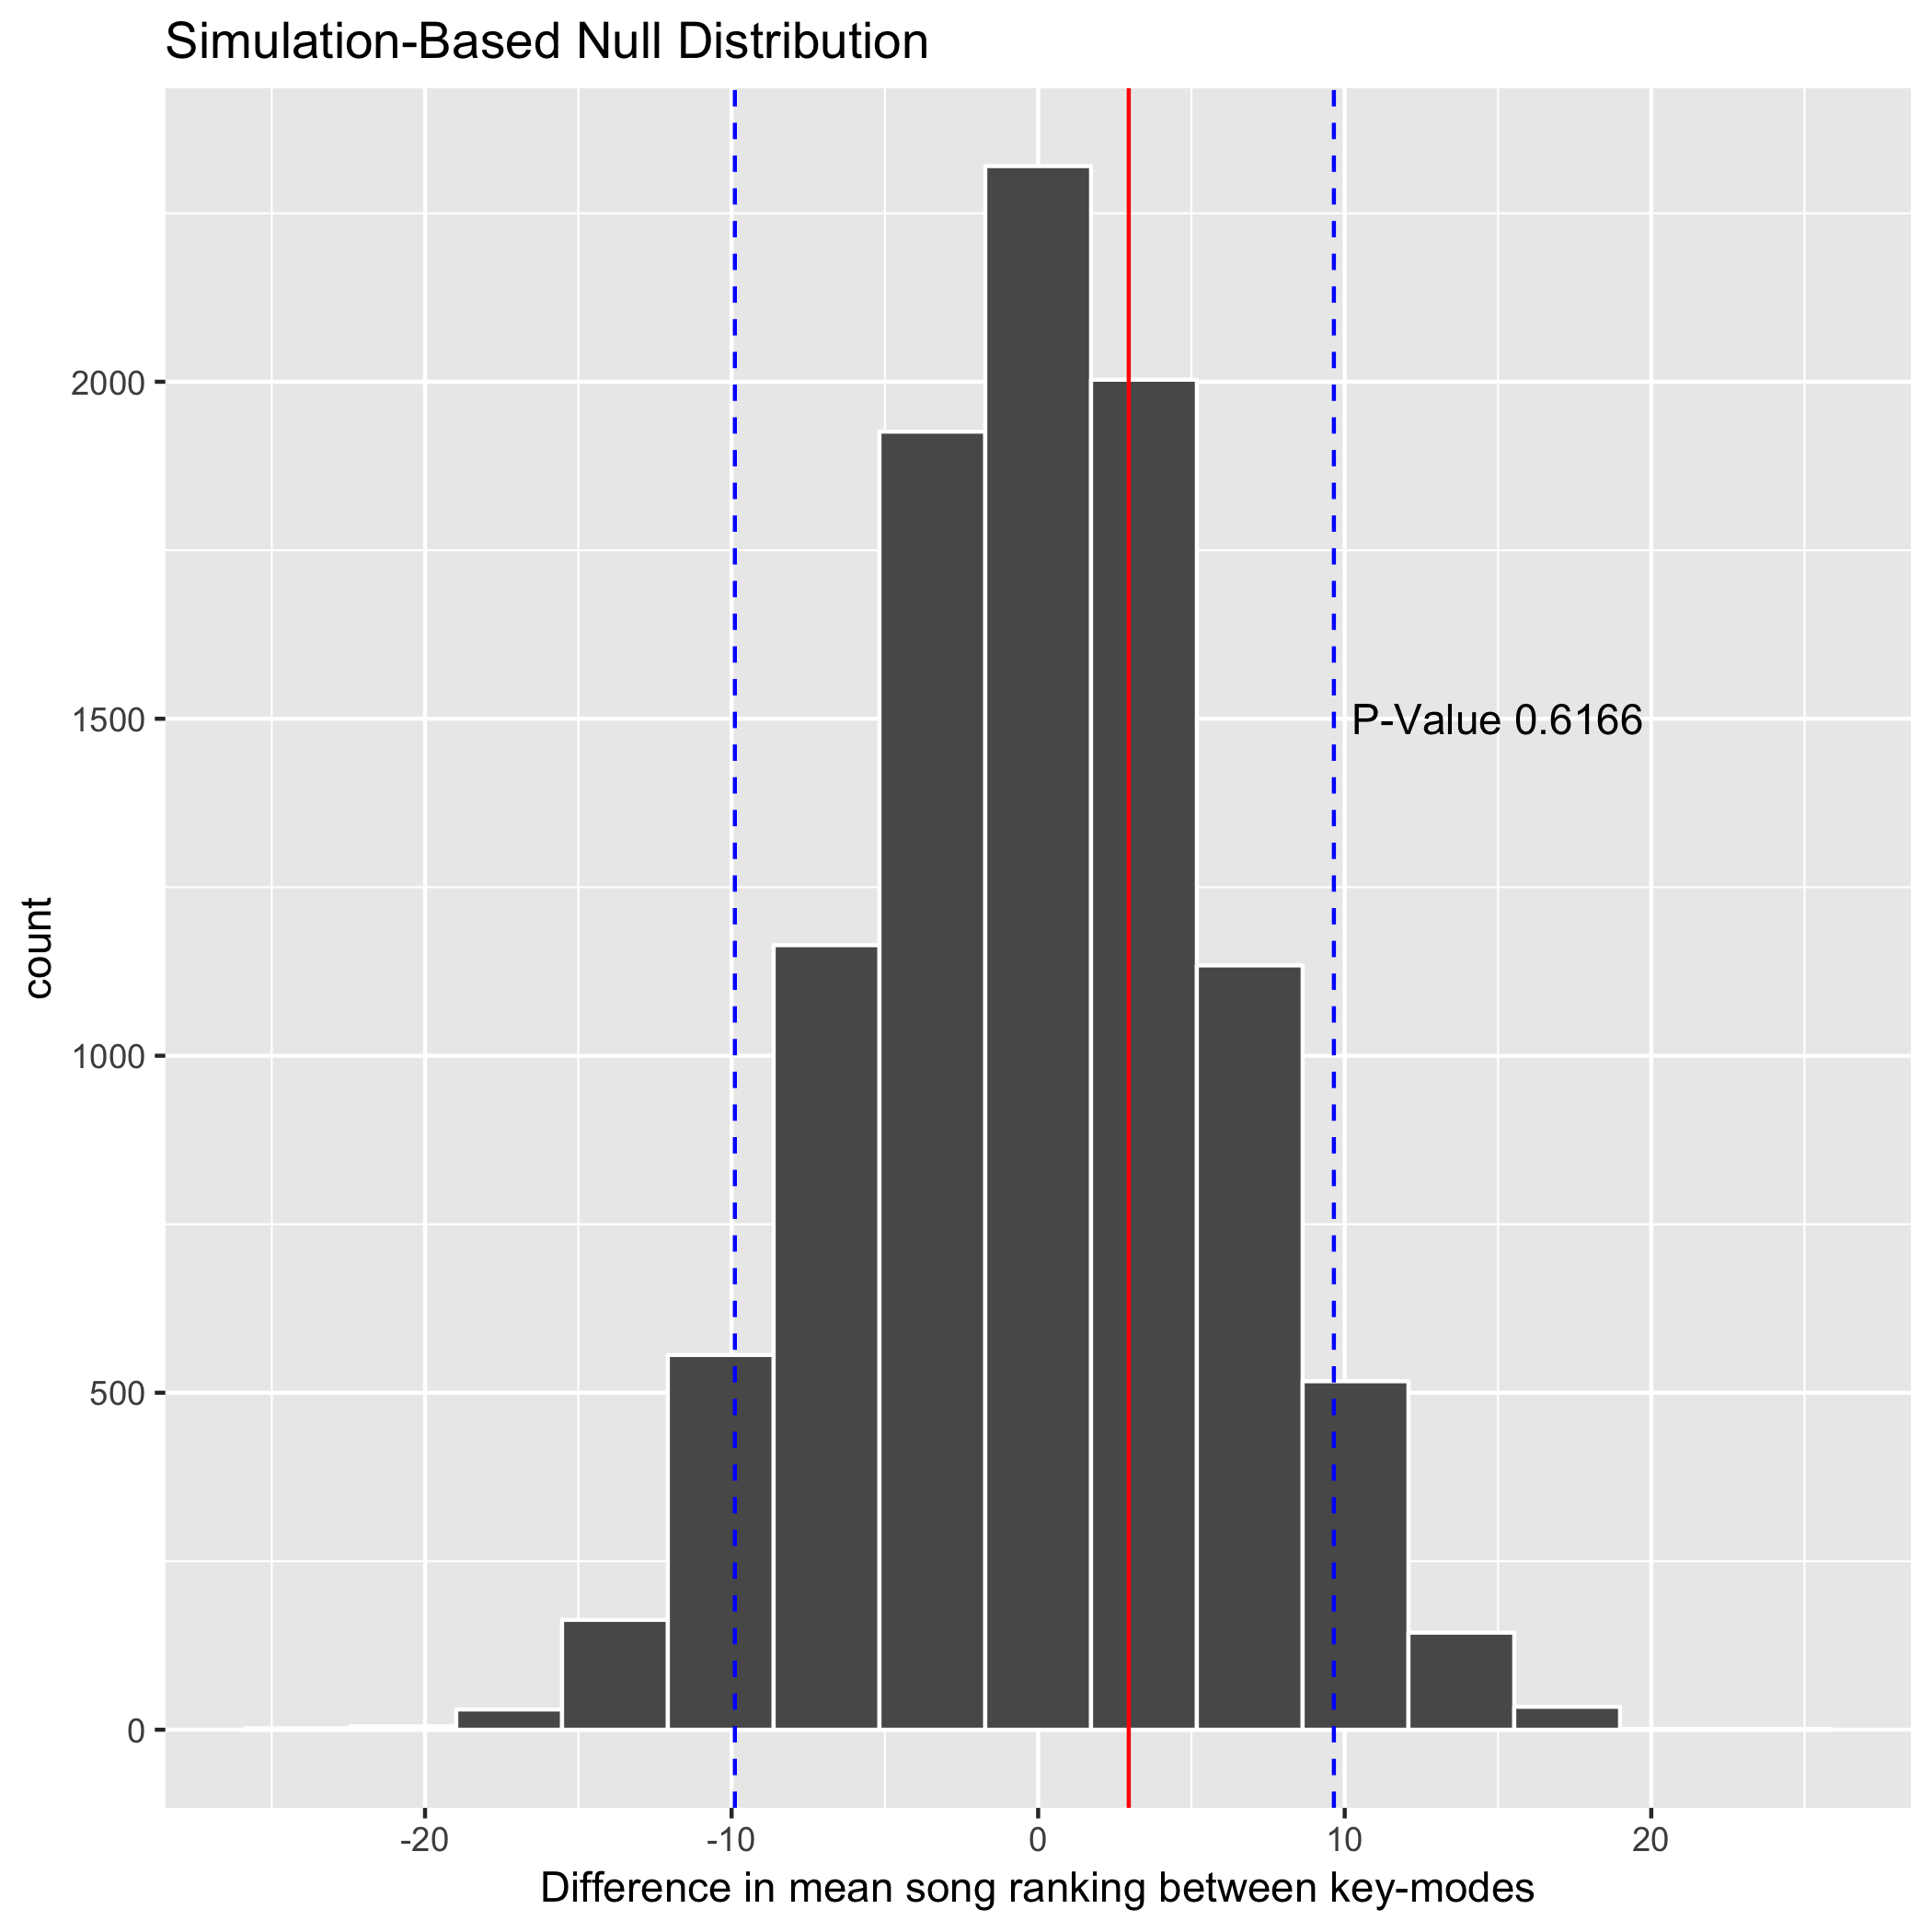
\includegraphics[width=0.8\linewidth]{../results/figure/Fig03_Test_Ddistr_Plot} \caption{Null distribution of rank by key-mode.  Error bars represent 90\% confidence intervals generated by TBD permutation}\label{fig:unnamed-chunk-5}
\end{figure}

\section{RESULTS:}\label{results}

\begin{itemize}
\tightlist
\item
  Our p-value is \textbf{$0.622$}. As our p-value is larger than the
  alpha (\textbf{$0.1$}), we do not reject the null hypothesis.
\end{itemize}

Our dataset is the top 100 songs which creates a sampling bias. Ideally,
we would be able to compare the proportions of songs in each key-mode
from the top 100 to the proportions of songs in each key-mode from a
random sample of Spotify songs.

This analysis is very limited due to time constraints, and we are only
taking into consideration one feature of the songs. We would like to
analyze all the features and their combinations to see how this affects
a song's popularity.

Given more time in the future, we would like to try a more in-depth
analysis and maybe try using a Decision Tree to consider all other song
features besides key-mode.

\subsection{REFERENCES}\label{references}

Top Spotify Tracks of 2017, Audio features of top Spotify songs -
Retrieved from:
\url{https://www.kaggle.com/nadintamer/top-tracks-of-2017}

Wikipedia Major and Minor - Retrieved from:
\url{https://en.wikipedia.org/wiki/Major_and_minor}

UBC MDS Statistical Inference Lecture 04 - Retrieved from:
\url{https://github.ubc.ca/MDS-2018-19/DSCI_552_stat-inf-1_students/blob/master/lectures/04_lecture-sim-estimation-wrap-up-and-hyp-test-intro.ipynb}

Wikipedia Spotify - Retriefed from:
\url{https://en.wikipedia.org/wiki/Spotify}


\end{document}
